\documentclass[svgnames,tikz]{standalone}
\usepackage{pgfplots}

\begin{document}
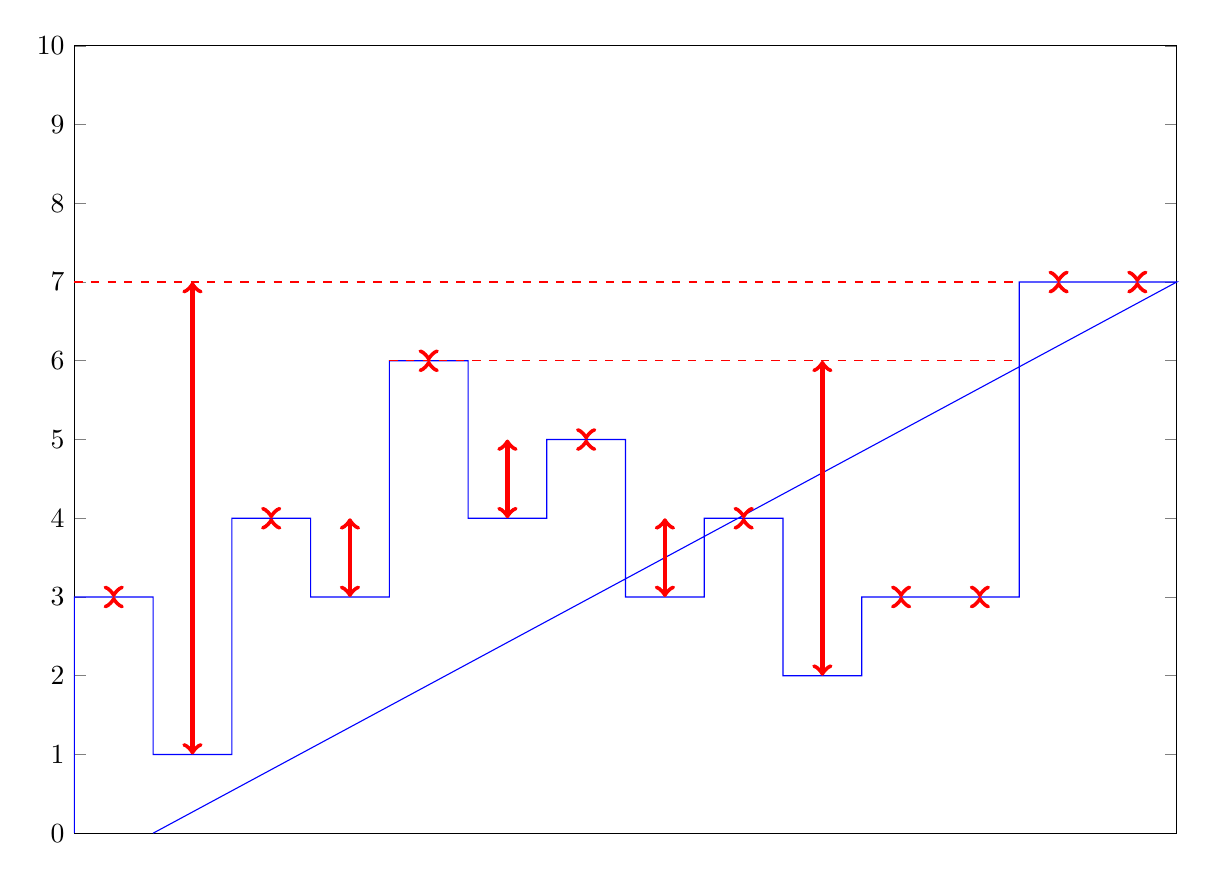
\begin{tikzpicture}[yscale=1]

\def\signalA{3,1,4,3,6,4,5,3,4,2,3,3,7,7}
\def\signalB{0,6,0,1,0,1,0,1,0,4,0,0,0,0}

\begin{axis}[
  x=1cm,y=1cm,
  xmin=0,xmax=14,
  ymin=0,ymax=10,
  xtick={\empty},ytick={},
]
\end{axis}



\draw[blue] (0,0) foreach[count=\x] \y in \signalA { |- (\x,\y) } -- (\x,0);

\foreach[evaluate=\i as \yA using {{\signalA}[\i]},
         evaluate=\i as \yB using {{\signalB}[\i]}] \i in {0,...,13}
{
  \draw[red,ultra thick] (\i,\yA) ++(+.5,0) edge[<->] ++(0,\yB);
}

\draw[dashed,red,thin]  (4,6) -- (12,6);
\draw[dashed,red,thin]  (0,7) -- (12,7);
\end{tikzpicture}
\end{document}
